\section{Normalization and Feature Processing}

\paragraph{Soil Properties:} 
Soil variables were normalized using property-specific transformations:
\begin{itemize}
    \item \textbf{Texture (COARSE, SAND, SILT, CLAY):} Min-Max scaling to range [0,1].
    \item \textbf{Density and pH:} Robust scaling for densities, Min-Max for pH.
    \item \textbf{Organic Matter and Nutrients:} Log-transform followed by robust scaling for organic carbon; log + standard scaling for total nitrogen; Min-Max for total carbon equivalents.
    \item \textbf{Cation Exchange and Fertility:} Robust scaling for CEC\_SOIL, CEC\_EFF, TEB; Min-Max for CEC\_CLAY, BSAT.
    \item \textbf{Salinity and Saturation:} Log-transform followed by robust scaling for ALUM\_SAT, ESP, GYPSUM, ELEC\_COND.
\end{itemize}

\subsection{Visualization of Normalization Effects}
The distributions of selected soil properties before and after normalization were compared to ensure consistency and scaling effectiveness.

\begin{figure}[H]
    \centering
    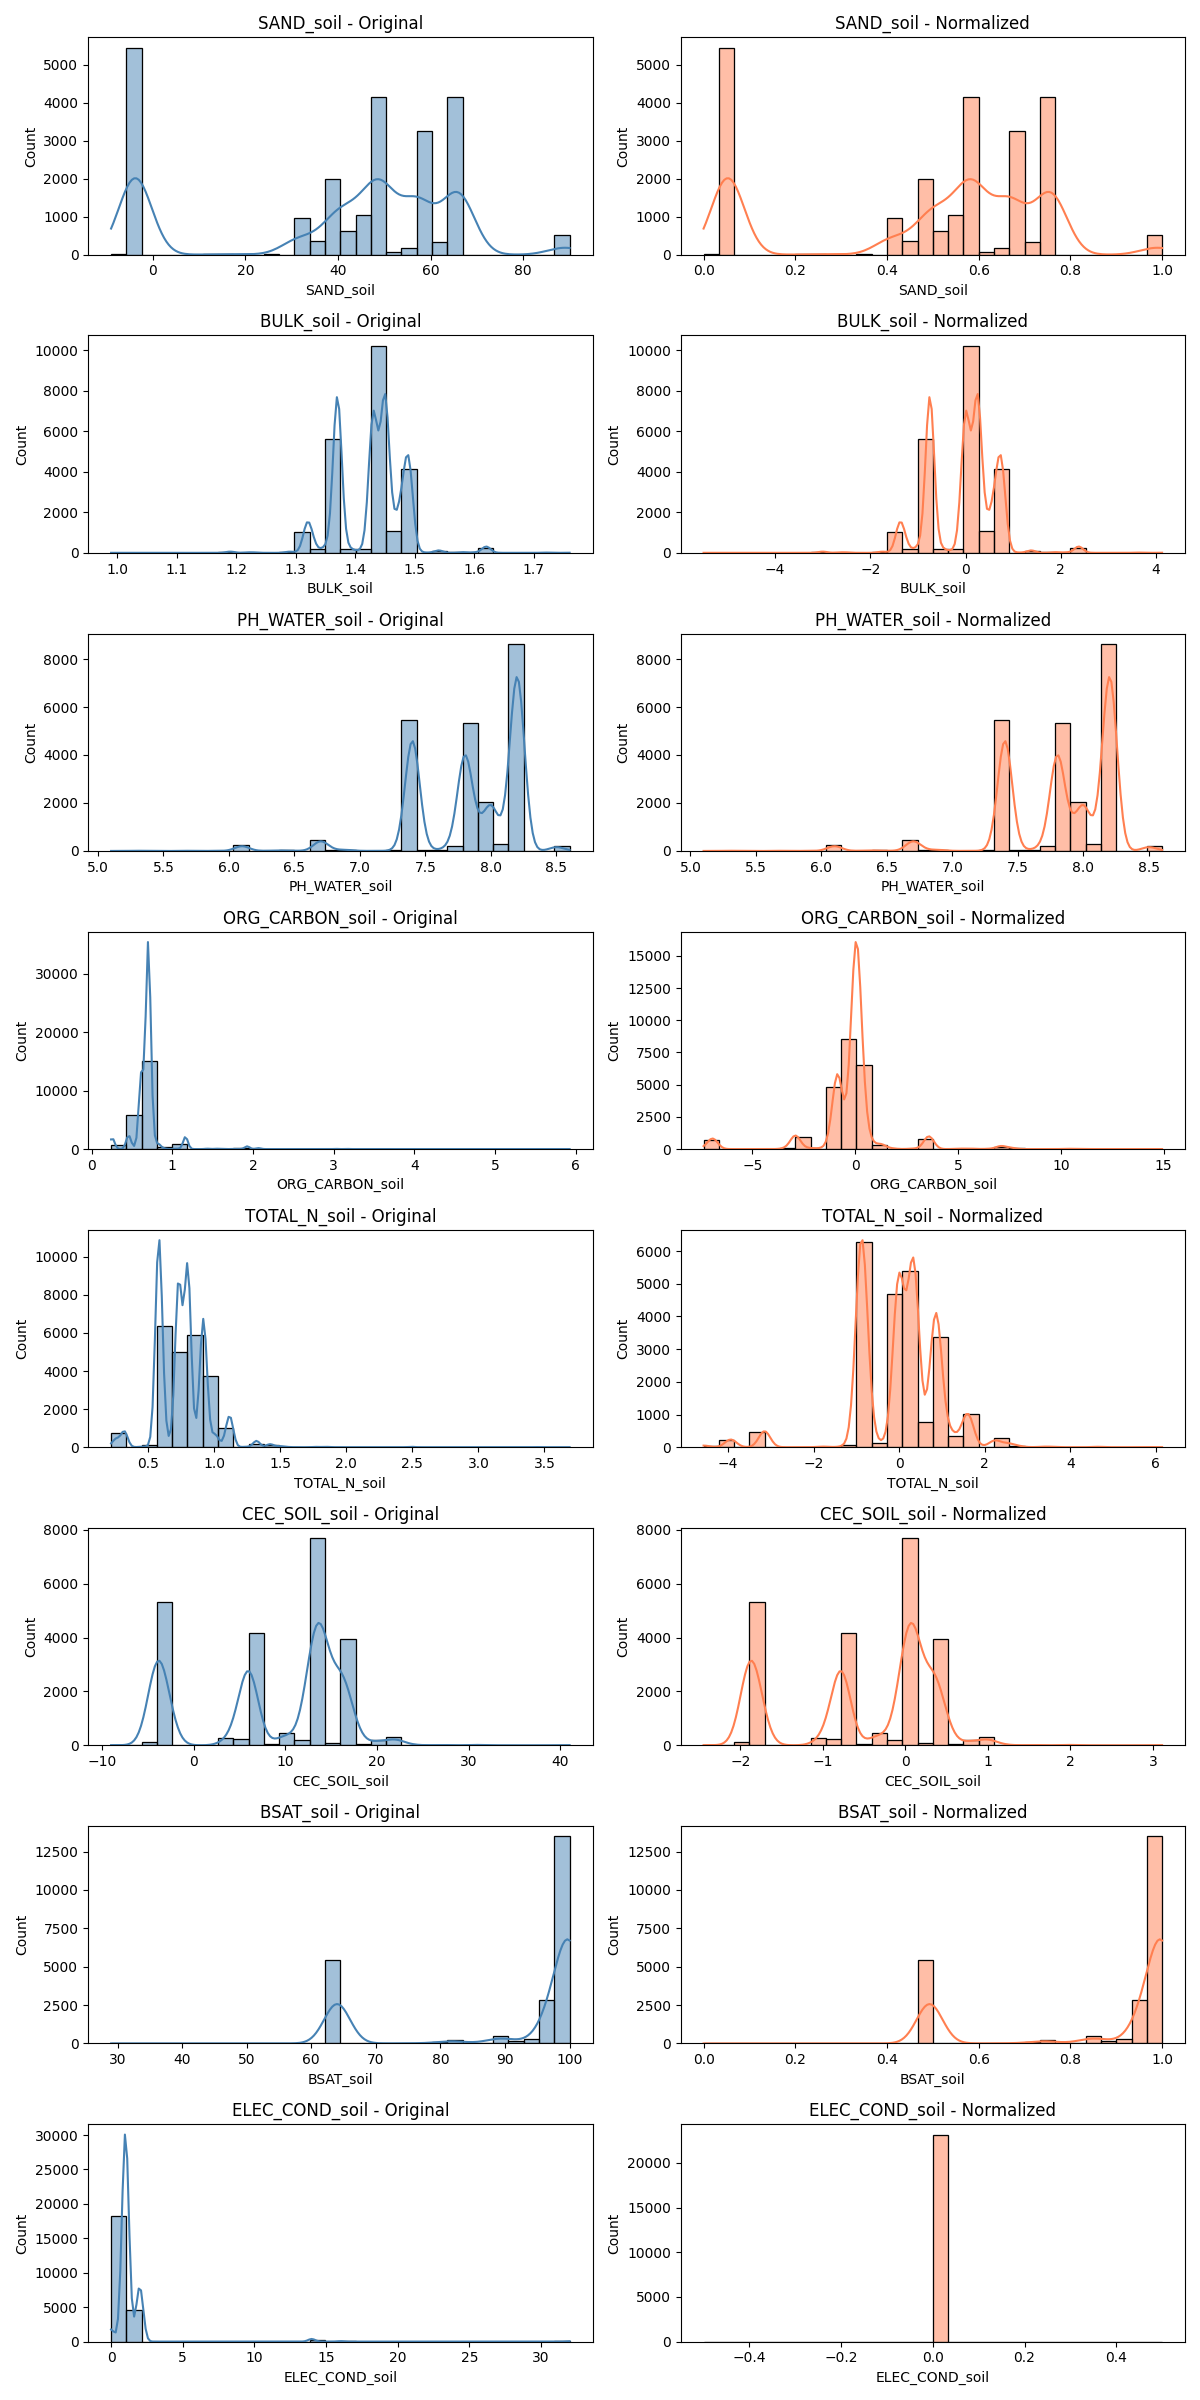
\includegraphics[width=0.6\textwidth]{images/MergedPreprocess/soil_normalization_comparison.png}
    \caption{Comparison of soil property distributions before and after normalization.}
    \label{fig:soil_normalization}
\end{figure}


\paragraph{Climate Features:} 
Temperature features were standardized (z-score), while precipitation features were log-transformed.

\paragraph{Elevation:} 
Standard scaling was applied to the elevation variable.

\paragraph{Land Cover Classification Code Harmonization}

The raw $\texttt{lcccode}$ column contains complex codes (e.g., \texttt{7001 // 8001}) which represent mixed, uncertain, or transitional land cover types. The separator (\texttt{//}) indicates a mixture between the two classes (e.g., Shrubland and Bare/Sparse vegetation). To handle this complexity for machine learning, the following steps were taken:

\textbf{Legend Integration}
The official legend files (\texttt{globcover\_LCCS\_legend\_africa.xls} and \texttt{globcover\_legend.xls}) were loaded to establish a mapping between the numeric codes and descriptive labels.

\begin{itemize}
    \item The $\texttt{LCCCode}$ was mapped to its descriptive label ($\texttt{LCCOwnLabel}$) using a dictionary.
    \item This process identified that certain codes were designated as ``Error'' in the $\texttt{LC}$ column of the legend, yet represented valid land cover types in the $\texttt{LCCOwnLabel}$ column (e.g., ``Closed forest''). This confirmed that these codes should be retained and mapped correctly.
\end{itemize}

\textbf{High-Level Mapping}
Given the 22 unique $\texttt{lcccode}$ values in the dataset, a high-level, simplified mapping was created to aggregate these codes into fundamental categories (e.g., ``Forests,'' ``Bare lands,'' ``Croplands,'' ``Vegetation,'' etc.). 
This step is crucial for reducing the complexity of the model's fire prediction.

\begin{table}[H]
    \centering
    \caption{Example of Landcover Transformation from \texttt{lcccode} to \texttt{lcc\_highlevel}}
    \label{tab:landcover_highlevel}
    \begin{tabular}{cc}
        \toprule
        \textbf{lcccode} & \textbf{lcc\_highlevel} \\
        \midrule
        7001 // 8001      & Water bodies \\
        7001 // 8001      & Water bodies \\
        7001 // 8001      & Water bodies \\
        21497-121340      & Forests \\
        7001 // 8001      & Water bodies \\
        \bottomrule
    \end{tabular}
\end{table}


\subsection{Saving the Normalized Data}
The final normalized dataset (\texttt{X\_train}) was saved in Parquet format for subsequent modeling steps.
